\let\negmedspace\undefined
\let\negthickspace\undefined
\documentclass[journal]{IEEEtran}
\usepackage[a5paper, margin=10mm, onecolumn]{geometry}
%\usepackage{lmodern} % Ensure lmodern is loaded for pdflatex
\usepackage{tfrupee} % Include tfrupee package

\setlength{\headheight}{1cm} % Set the height of the header box
\setlength{\headsep}{0mm}     % Set the distance between the header box and the top of the text

\usepackage{gvv-book}
\usepackage{gvv}
\usepackage{cite}
\usepackage{amsmath,amssymb,amsfonts,amsthm,mathtools}
\usepackage{algorithmic}
\usepackage{graphicx}
\usepackage{textcomp}
\usepackage{xcolor}
\usepackage{txfonts}
\usepackage{listings}
\usepackage{enumitem}
\usepackage{mathtools}
\usepackage{gensymb}
\usepackage{comment}
\usepackage[breaklinks=true]{hyperref}
\usepackage{tkz-euclide} 
\usepackage{listings}
\def\inputGnumericTable{}                                 
\usepackage[latin1]{inputenc}                                
\usepackage{color}                                            
\usepackage{array}                                            
\usepackage{longtable}                                       
\usepackage{calc}                                             
\usepackage{multirow}                                         
\usepackage{hhline}                                           
\usepackage{ifthen}                                           
\usepackage{lscape}
\begin{document}

\bibliographystyle{IEEEtran}
\vspace{3cm}

\title{3.3.2.14}
\author{EE24BTECH11024 - G. Abhimanyu Koushik
}
% \maketitle
% \newpage
% \bigskip
{\let\newpage\relax\maketitle}

\renewcommand{\thefigure}{\theenumi}
\renewcommand{\thetable}{\theenumi}
\setlength{\intextsep}{10pt} % Space between text and floats

\textbf{Question:}\\
Two sides of a triangle are of length $5cm$ and $1.5cm$. The length of the third side of the triangle cannot be
\\
\begin{enumerate}[label=\alph*.]
	\item $3.6cm$
	\item $4.1cm$
	\item $3.8cm$
	\item $3.4cm$
\end{enumerate}
\textbf{Solution:}
\begin{table}[h!]    
  \centering
  \begin{tabular}[12pt]{ |c|c|c|}
    \hline
    \textbf{Symbol} & \textbf{Value} & \textbf{Description} \\
    \hline
    $\vec{A}$ & \myvec{6\\5} & First point\\
    \hline 
    $\vec{B}$ & \myvec{-4\\3} & Second point\\
    \hline
    $\vec{Y}$ & \myvec{0\\$y$} & Point on Y-Axis equidistant from A and B\\
    \hline
    \end{tabular}

  \caption{Variables Used}
  \label{tab10.5.3.9.1}
\end{table}\\
For any triangle the difference of length of two sides should not be greater than the third side. 
\begin{align}
	\abs{a-b} \geq c\\
	3.5cm \geq c
\end{align}
$c$ cannot be $3.4cm$
\begin{figure}[h!]
   \centering
   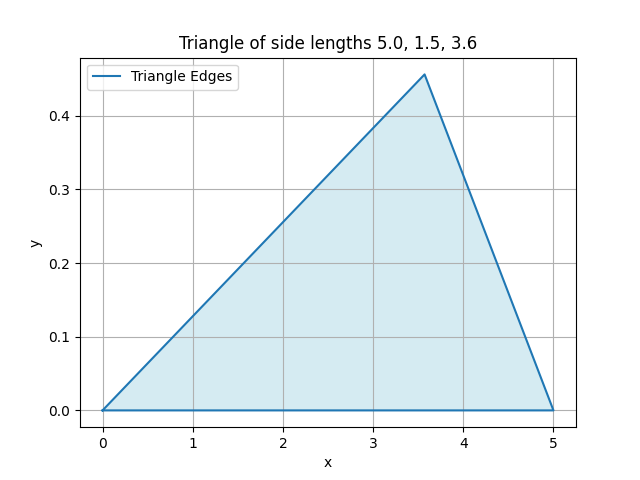
\includegraphics[width=0.7\linewidth]{figs/fig1.png}
   \caption{Triangle with sides $5cm$, $1.5cm$, and $3.6cm$}
\end{figure}

\setcounter{figure}{1} % Force figure numbering to 2
\begin{figure}[h!]
   \centering
   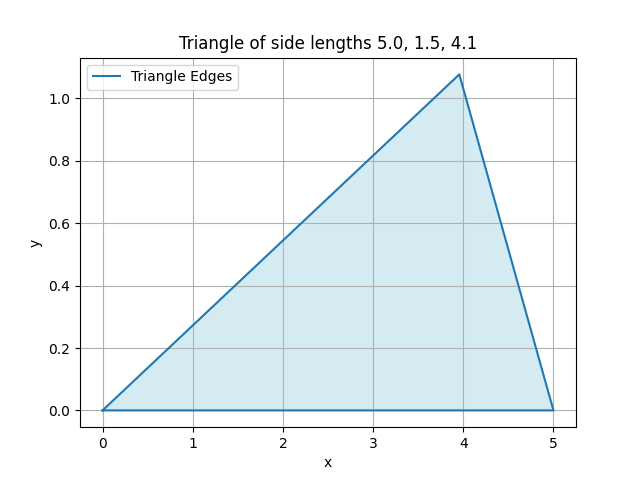
\includegraphics[width=0.7\linewidth]{figs/fig2.png}
   \caption{Triangle with sides $5cm$, $1.5cm$, and $4.1cm$}
\end{figure}

\setcounter{figure}{2} % Force figure numbering to 3
\begin{figure}[h!]
   \centering
   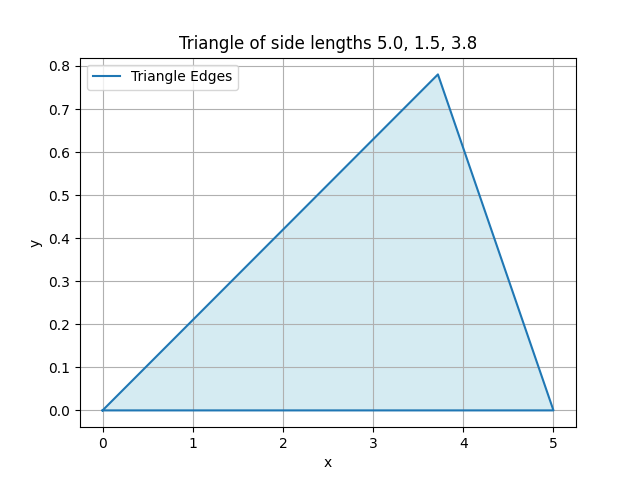
\includegraphics[width=0.7\linewidth]{figs/fig3.png}
   \caption{Triangle with sides $5cm$, $1.5cm$, and $3.8cm$}
\end{figure}

\setcounter{figure}{3} % Force figure numbering to 4
\begin{figure}[h!]
   \centering
   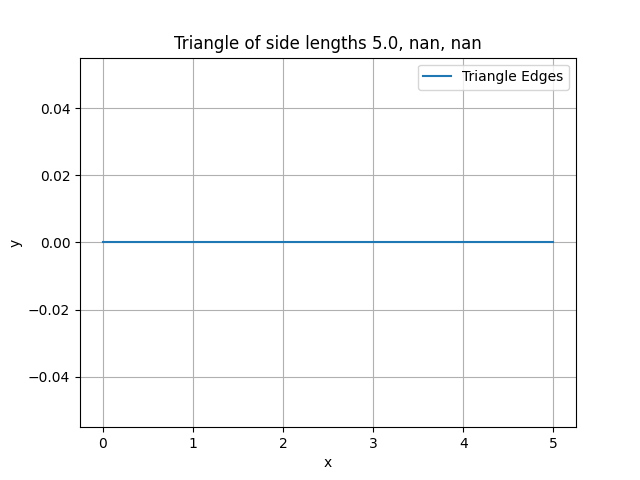
\includegraphics[width=0.7\linewidth]{figs/fig4.png}
   \caption{Code giving an error (only a line) as the triangle cannot exist}
\end{figure}

\end{document}
